\documentclass[margin=5mm]{standalone}
\usepackage[dvipsnames]{xcolor}
\usepackage{pgfplots}
\usepackage{tikz}
\usepackage[tikz]{ocgx2}

\pgfplotsset{compat=1.18}
\begin{document}

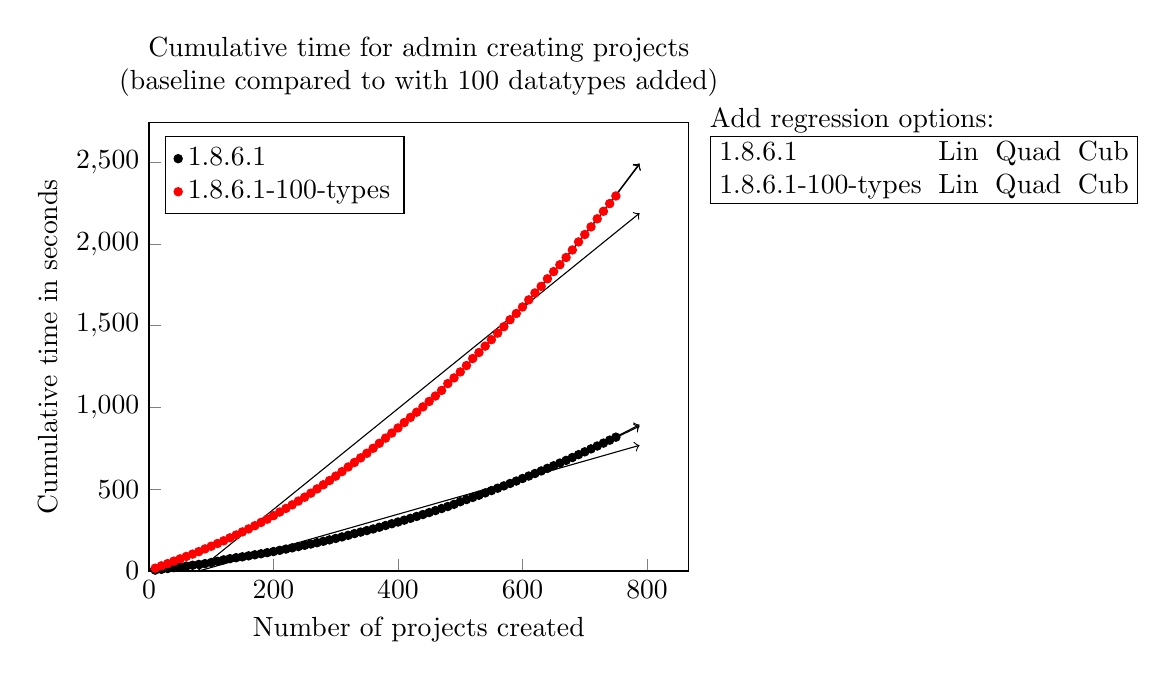
\begin{tikzpicture}
    \begin{axis}[
        align = center,
        legend pos = north west,
        legend cell align = left,
        xlabel = Number of projects created,
        ylabel = Cumulative time in seconds,
        xtick pos = left,
        ytick pos = left,
        scaled ticks = false,
        xmin = 0,
        ymin = 0,
        title = {Cumulative time for admin creating projects (baseline compared to with 100 datatypes added)},
        title style = {text width = 0.8\textwidth},
        legend entries={\switchocg{1.8.6.1}{1.8.6.1},\switchocg{1.8.6.1-100-types}{1.8.6.1-100-types}}]
        \begin{scope}[ocg = {ref = 1.8.6.1-Lin, status = invisible}]
            \plot[domain=0:788,->,forget plot] (\x,{-87.2929405405404708062633289955556392669677734375 + 1.085280896159316998961230638087727129459381103515625*(\x)^1});
        \end{scope}
        \begin{scope}[ocg = {ref = 1.8.6.1-Quad, status = invisible}]
            \plot[domain=0:788,->,forget plot] (\x,{8.406666790077711226558676571585237979888916015625 + 0.339569670206447626892298785605817101895809173583984375*(\x)^1 + 0.000981198981516933667335056412639460177160799503326416015625*(\x)^2});
        \end{scope}
        \begin{scope}[ocg = {ref = 1.8.6.1-Cub, status = invisible}]
            \plot[domain=0:788,->,forget plot] (\x,{2.454060125879252485248116499860771000385284423828125 + 0.43055878463904451169952380951144732534885406494140625*(\x)^1 + 0.0006838659813072204586570368434195188456214964389801025390625*(\x)^2 + 0.0000002608184212365905082941955166198066962124357814900577068328857421875*(\x)^3});
        \end{scope}
        \begin{scope}[ocg = {ref = 1.8.6.1, status = visible}]
            \addplot[
                only marks,
                color = black,
                mark = *,
                mark size = 1.5 pt
            ]coordinates {(10,5.181)(20,9.932)(30,14.881)(40,20.123)(50,25.02)(60,30.031)(70,34.85)(80,39.834)(90,44.847)(100,51.662)(110,59.247)(120,67.972)(130,75.059)(140,80.906)(150,86.42)(160,92.362)(170,98.746)(180,105.021)(190,111.886)(200,118.524)(210,126.164)(220,133.744)(230,141.297)(240,149.019)(250,156.8)(260,164.628)(270,172.824)(280,181.453)(290,189.979)(300,198.656)(310,207.964)(320,217.805)(330,228.137)(340,237.47)(350,246.934)(360,256.63)(370,267.22)(380,277.667)(390,288.631)(400,299.213)(410,310.469)(420,321.791)(430,333.244)(440,344.794)(450,356.842)(460,368.906)(470,381.477)(480,393.973)(490,407.162)(500,423.23)(510,436.332)(520,449.602)(530,462.802)(540,477.047)(550,491.119)(560,505.719)(570,520.085)(580,534.784)(590,549.737)(600,565.199)(610,580.198)(620,595.594)(630,611.291)(640,627.266)(650,643.036)(660,659.543)(670,675.931)(680,693.403)(690,710.964)(700,728.319)(710,746.165)(720,763.821)(730,781.559)(740,799.561)(750,817.831)};
        \end{scope}
        \begin{scope}[ocg = {ref = 1.8.6.1-100-types-Lin, status = invisible}]
            \plot[domain=0:788,->,forget plot] (\x,{-239.649089009008577022541430778801441192626953125 + 3.079963567567566951055368917877785861492156982421875*(\x)^1});
        \end{scope}
        \begin{scope}[ocg = {ref = 1.8.6.1-100-types-Quad, status = invisible}]
            \plot[domain=0:788,->,forget plot] (\x,{8.5057542835989305984867314691655337810516357421875 + 1.146289463988806378580420641810633242130279541015625*(\x)^1 + 0.002544308031024685758103576205257922993041574954986572265625*(\x)^2});
        \end{scope}
        \begin{scope}[ocg = {ref = 1.8.6.1-100-types-Cub, status = invisible}]
            \plot[domain=0:788,->,forget plot] (\x,{12.1291984326794430870677388156764209270477294921875 + 1.0909029765355453545083719291142188012599945068359375*(\x)^1 + 0.002725299247262482661702254205238205031491816043853759765625*(\x)^2 + -0.000000158764224769997388530214424938458162017695940448902547359466552734375*(\x)^3});
        \end{scope}
        \begin{scope}[ocg = {ref = 1.8.6.1-100-types, status = visible}]
            \addplot[
                only marks,
                color = red,
                mark = *,
                mark size = 1.5 pt
            ]coordinates {(10,16.959)(20,31.404)(30,44.983)(40,60.136)(50,73.981)(60,88.724)(70,102.943)(80,118.136)(90,134.787)(100,151.215)(110,167.786)(120,184.424)(130,202.286)(140,219.837)(150,238.729)(160,257.012)(170,276.55)(180,296.679)(190,316.485)(200,337.877)(210,360.207)(220,382.354)(230,404.186)(240,427.428)(250,450.874)(260,475.548)(270,501.764)(280,526.881)(290,552.655)(300,579.678)(310,607.232)(320,635.709)(330,663.304)(340,691.416)(350,719.738)(360,750.031)(370,780.496)(380,812.257)(390,842.978)(400,874.208)(410,907.091)(420,938.977)(430,970.609)(440,1002.949)(450,1036.305)(460,1069.372)(470,1103.397)(480,1145.569)(490,1180.193)(500,1216.622)(510,1255.65)(520,1298.698)(530,1335.371)(540,1374.502)(550,1413.932)(560,1453.916)(570,1493.211)(580,1535.928)(590,1574.029)(600,1613.807)(610,1657.29)(620,1699.586)(630,1739.983)(640,1786.197)(650,1830.202)(660,1872.109)(670,1916.333)(680,1962.194)(690,2011.516)(700,2056.709)(710,2103.404)(720,2152.829)(730,2198.778)(740,2245.706)(750,2292.439)};
        \end{scope}
    \end{axis}
    \begin{scope}
        \addtolength{\tabcolsep}{-0.3em}
        \node [below right, shape=rectangle, align=left](regressiontable) at (7,6) {
            Add regression options: \\
            \begin{tabular}{|llll|}
                \hline
                1.8.6.1 & \switchocg{1.8.6.1-Lin}{Lin} & \switchocg{1.8.6.1-Quad}{Quad} & \switchocg{1.8.6.1-Cub}{Cub} \\
                1.8.6.1-100-types & \switchocg{1.8.6.1-100-types-Lin}{Lin} & \switchocg{1.8.6.1-100-types-Quad}{Quad} & \switchocg{1.8.6.1-100-types-Cub}{Cub} \\
                \hline
            \end{tabular}
        };
    \end{scope}
\end{tikzpicture}

\end{document}